\documentclass[10pt,a4paper]{article}
\usepackage[latin1]{inputenc}
\usepackage{amsmath}
\usepackage{amsfonts}
\usepackage{amssymb}
\usepackage{graphicx}
\usepackage{float}
\usepackage{bm}
\title{Week 6 exercises}
\begin{document}
	\maketitle
	\begin{enumerate}
		\item The linear probability model for binary response is simply $ P(y = 1) =   \pi_i = \bm{x_i'\beta} = \beta_{0i} + 
		\beta_{1i} x_{1i}  + \dots + \beta_{ni} x_{ni}   $ and require the restriction that $ 0  \leq  \bm{X'\beta}  \leq 1 $ 
		\item In the GLM we combine the probability output to the linear prediction through a function \textit{h} called \textit{response function} that it is a cumulative distribution function with co domain in [0,1]. In formula we can express the GLM as $$ P(y = 1) =   \pi_i = h(\eta_i) = h(\mathbf{x_i'\beta}) = h(\beta_{0i} + 
		\beta_{1i} x_{1i}  + \dots + \beta_{ni} x_{ni})  $$\\$ g = h^{-1} $ is the \textit{link function} and it is used to calculate the linear predictor in function of probability: $ \eta_i = g(\pi_i) $ 
		The logit model use as response function the logistic function: $$ \pi = h(\eta) = \dfrac{e^\eta}{1 + e^\eta} $$. The linear predictor returns the log odds $$ \mathbf{x_i'\beta} = \beta_{0i} + 
		\beta_{1i} x_{1i}  + \dots + \beta_{ni} x_{ni} =  \pi_i = \log\left(\dfrac{\pi}{1 - \pi}\right)   $$.
		The probit model use instead a normal distribution cumulative function.
		The c-log-log model use as response function the extreme minimum-value cumulative
		distribution function
		$$ h(\eta) = 1 - e^{-e^\eta}$$ with the following link function $$ g(\pi) = \log(- \log( 1 - \pi )) $$
		\item 
		\begin{figure}[H]
			\centering
			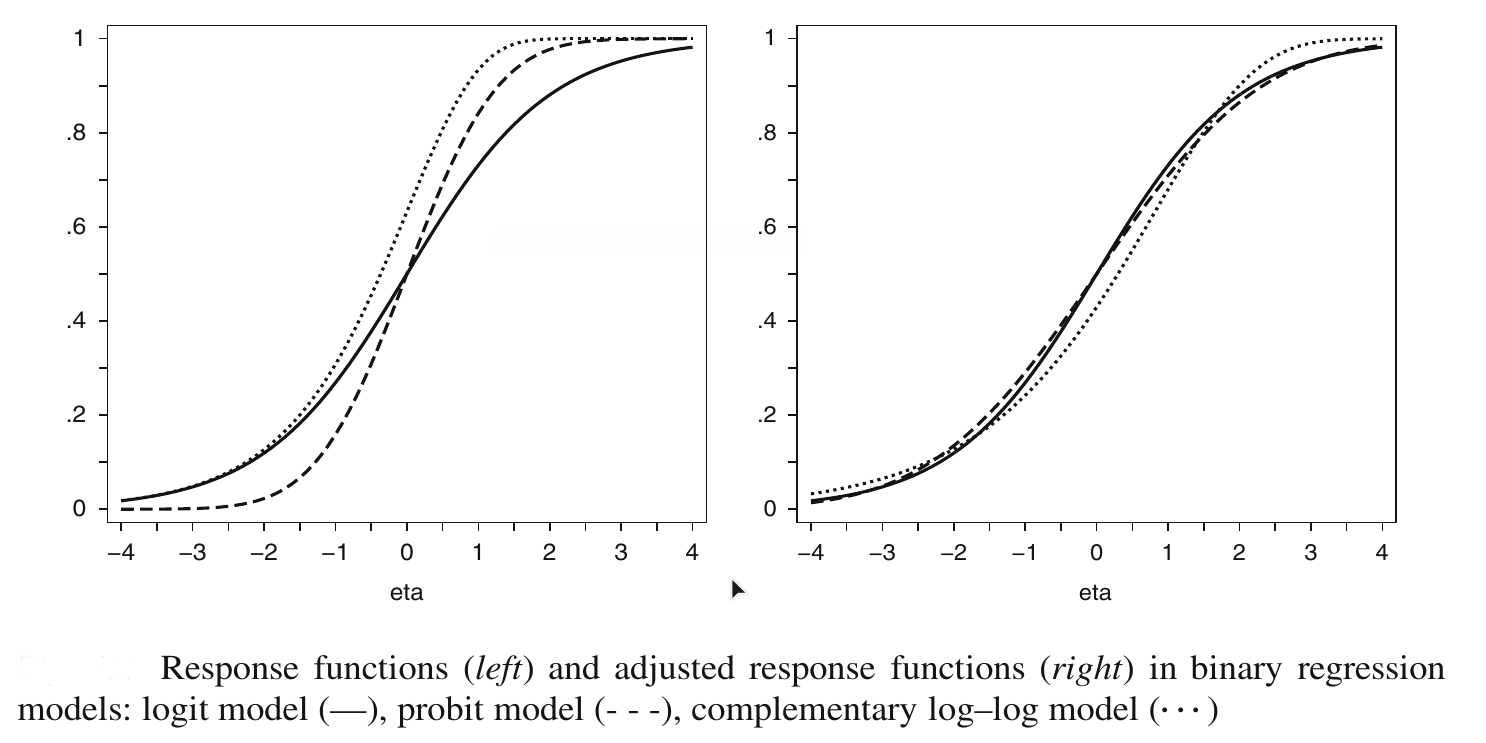
\includegraphics[width=0.7\linewidth]{plot_comparison_response_functions}
			\label{fig:plotcomparisonresponsefunctions}
		\end{figure}
		From the latter plot we can note that the \textit{probit} and \textit{logit} are symmetric around the 0 while the c-log-log is not symmetric. The c-log-log is similar to the logit but tend more speedly to one. If we do a comparison with the same variance between the logit and probit we have that the coefficients differ for a values of $ \frac{\pi}{3} = 1.814 $
		\item With a latent continuous variable we use the standard normal distribution for the errors because we don't know the variance of the latent variable so the new coefficients are $ \tilde{\beta} = \frac{\beta}{\sigma} $. We can't calculate the original $ \beta $ since doesn't know $ \sigma $ but the ratio between coefficients are constants $ \dfrac{\tilde{\beta}_i}{\tilde{\beta}_j} = \dfrac{\beta_i}{\beta_j}$ 
		\item In the logit model if increase $ x_k $ by 1 we have an increments on the odds by $ e^\beta $ while the increment of probability is not the same in every point. \\ In the probit model we have an increment equal to $ \phi^{-1}(\beta) $
		\end{enumerate}
		\subsection*{Solution to applied exercise}
		\begin{enumerate}
			\item 		$$ \eta = 0.42 + 0.06 \cdot kidsge6 - 1.44 \cdot kidslt6 - 0.09 \cdot age + 0.21 \cdot exper - 0.0031 \cdot exper^2 + 0.22 \cdot educ - 0.021 \cdot nwifeinc$$
			$$
			P(y = 1) =
			\hat{\pi} = h(\hat{\eta}) =   \dfrac{e^{\hat{\eta}}}{1 + e^{\hat{\eta}}} $$
			\item $$ 0.42 + 0.06 \cdot 0 - 1.44 \cdot 0 - 0.09 \cdot 40 + 0.21 \cdot 0 - 0.0031 \cdot 0 + 0.22 \cdot 10 - 0.021 \cdot 0 = -0.98$$
			\item one year of more eduction when all the other variables are the same is a multiplicative effect of $ e^{0.22} $
			\item The probability is 0.27
			\item -0.0174
			\item 0.046
			\item $ 0.22 * 0.5^2 =  0.055 $
			\item The probit coefficients are obtained by dividing by 1.84
		\end{enumerate}

\end{document}